\documentclass[11pt]{amsart}
\usepackage{geometry}                % See geometry.pdf to learn the layout options. There are lots.
\geometry{a4paper}                   % ... or a4paper or a5paper or ... 
%\geometry{landscape}                % Activate for for rotated page geometry
\usepackage[parfill]{parskip}    % Activate to begin paragraphs with an empty line rather than an indent
\usepackage{graphicx}
\usepackage{amssymb}
\usepackage{epstopdf}
\usepackage{newtxtext, newtxmath}
\DeclareGraphicsRule{.tif}{png}{.png}{`convert #1 `dirname #1`/`basename #1 .tif`.png}

\title{Time-Series Characteristics of Live Cattle Futures}
\author{2025...}
%\date{}                                           % Activate to display a given date or no date

\begin{document}
\maketitle
\section{Introduction}

Beef is a key source of protein in the human food chain, its price is therefore
a matter of both economic, commercial and national interest. It is estimated
that around 62 million tonnes of beef was produced worldwide in 2025 (US
Department of Agriculture, 2025).

Unlike sheep, cattle are sufficiently invariate to allow for the application of
standardised futures contracts to their trade. The S\&PGSCI Live Cattle Futures
index is based on live cattle futures traded on the Chicago Mercantile Exchange
for delivery to US auctions, reweighted to reflect global production. It is
therefore described as a global index. The particular index under examination
uses the contract for nearest delivery, and is analogous (though not identical
to) a spot market. 

This study will examine the statistical characteristics of this index, and
attempt to create a model of its price movements. 

\section{Stationarity}

4024 daily close prices were obtained through Google Finance, corresponding to 
the period 2010-01-01 to 2026-01-01. 

\begin{figure}
\centering
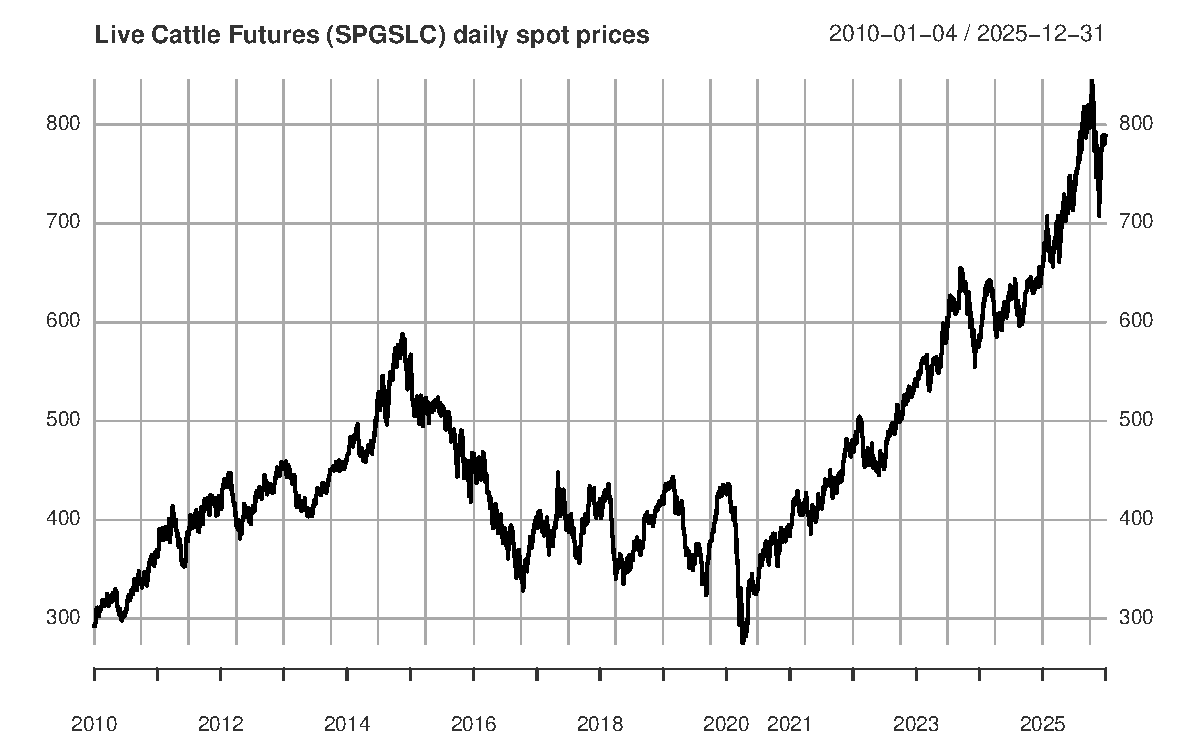
\includegraphics[width=\linewidth]{../cattle.pdf}
\caption{Live cattle prices}
\end{figure}


%\subsection{}



\end{document}  
